% !TeX encoding = UTF-8
% Use XeLaTeX to compile it
%
% Эта работа распространяется на условиях лицензии Creative Commons Attribution-Noncommercial-Share Alike 3.0 New Zealand License.
% Краткое описание лицензии есть тут: http://creativecommons.org/licenses/by-nc-sa/3.0/nz/deed.ru
% Полное — там же.
% Эту книгу можно невозбранно распространять и изменять, но только соблюдая следующие условия:
% сохраняя лицензию и не вводя дополнительных ограничений, бесплатно
% и указывая авторство как оригинальной части, так и изменённой.
% Автор оригинального английского текста — Jason R Briggs http://jasonrbriggs.com/
% Автор перевода — Егор Кочетов <Egor.Kochetoff@gmail.com>
%
% This work is licensed under the Creative Commons Attribution-Noncommercial-Share Alike 3.0 New Zealand License.
% To view a copy of this license, visit http://creativecommons.org/licenses/by-nc-sa/3.0/nz
% or send a letter to Creative Commons, 171 Second Street, Suite 300, San Francisco, California, 94105, USA.
%

\chapter{Немного компьютерной графики}\label{ch:abitgraphic}

Когда просишь черепашку что-нибудь нарисовать, сталкиваешь с одной проблемой. Дело в том… что черепашка… … очень… … … медленная.

Даже если попросить черепашку рисовать так быстро, как возможно, она всё равно будет делать это медленнее, чем хотелось бы. Для черепах вообще это не проблема — у них полно времени, — но вот рисовать на экране нужно быстрее, чтобы изображение не дёргалось и не замирало. Вспомни на секунду, какие бывают игры для компьютера или для переносных устройств типа Gameboy, Nintendo; для мобильных телефонов. У них бывает двухмерная графика: какие-нибудь плоские фигурки, которые движутся по плоскому полю — именно такая графика у большинства игр для телефонов, например. Бывает псевдо-трёхмерная графика: когда фигурки и поле нарисованы не плоскими, а как будто мы их видим сверху сбоку, под углом. Двигаются при этом они тоже по плоскому полю, и такие игры почти и не отличаются от двухмерных. А бывают игры, в которых изображение похоже на реальный трёхмерный мир — обычно это игры для компьютера, но и в телефонах бывают.

У всех этих видов графики общее одно: рисовать на экране компьютера надо очень быстро. Сейчас объясню, почему. Вот представь, что ты рисуешь на бумаге свой маленький мультфильм. Для этого нужна стопка чистой бумаги — ну и карандаш, например. На первом листочке из стопки сбоку надо нарисовать какую-нибудь картнику — допустим, кота. На втором листочке — точно такую же картинку, но чуть пошевелившую хвостом. На следующей картинке хвост кота должен двинуться ещё дальше — и так далее. Потом надо держать эту стопку бумаги за тот край, где нет рисунков, а другой рукой пролистывать быстро стопку, и тогда будет казаться, что кот в самом деле шевелит хвостом. Именно так работает вся анимация: фильмы, мультики, игры в компьютере. Быстро-быстро (по крайней мере 24 раза в секунду) одна картинка, или один кадр, сменяет другой, похожий. Черепашка с такими скоростями рисовать просто не умеет.

Трёхмерная графика рисуется похожим образом, хотя и по-другому. Там точно так же часто-часто сменяются кадры, но вот что именно должно быть нарисовано в каждом кадре высчитывается отдельно (достаточно хитрым способом). К тому моменту, как черепашка бы только посчитала, что нужно нарисовать в очередном кадре, уже было бы пора рисовать следующий.

\begin{center}
\includegraphics*[width=100mm]{../en/turtle1.eps}
\end{center}

\section{Рисуем быстро}

В каждом языке программирования есть свой способ рисовать на экране. Некоторые способы позволяют рисовать быстро, некототрые — медленно, так что программисты, которые пишут игры, пользуются только подходящими языками программирования.

В Питоне можно рисовать несколькими способами (включая ту же черепашку), но быстрее всего рисуют на экране библиотеки, которые не устанавливаются сразу вместе с Питоном (потому что они нужны совсем не всем). Я про них не буду рассказывать, потому что они сложные, и только после пары лет программирования будет вообще понятно, как ими пользоваться.

К счастью, с Питоном устанавливается модуль, который вполне можно использовать, чтобы рисовать на экране несложные элементы управления — например, кнопки и окна. Пожалуй даже, этот способ рисует настолько быстро, что его можно назвать быстрой черепашкой.

\begin{center}
\includegraphics*[width=100mm]{../en/turtle2.eps}
\end{center}

Модуль этот называется \code{tkinter}\index{модули!tkinter} (сокращение от 'Tk interface', что бы это ни значило). При помощи этого модуля можно создавать полноценные программы (например, вполне получится создать редактор текста), и ещё можно рисовать несложные картинки. Сложные тоже можно, но это долго программировать, и они будут медленно рисоваться на экране.

Можно создать программу, которая рисует на экране кнопку, вот так:

\begin{listing}
\begin{verbatim}
1. >>> from tkinter import *
2. >>> tk = Tk()
3. >>> btn = Button(tk, text="жми сюда")
4. >>> btn.pack()
\end{verbatim}
\end{listing}

В первой строчке мы говорим Питону импортировать всё из модуля \code{Tk}, чтобы использовать оттуда потом функции. Потом, во второй строке, мы тут же и используем одну функцию: \code{Tk()}, она нам создаёт окно, которое мы сохраняем в переменную \code{tk} и которое тут же появляется на экране. В третьей строке мы создаём кнопку функцией \code{Button}, она тоже из модуля \code{Tk}, и её записываем в переменную \code{btn}. Функции создания кнопки мы говорим, для какого окна её создавать и что должно быть написано на кнопке (для этого мы передаём \emph{именованный параметр} \code{text}). И наконец, в четвёртой строке мы отправляем кнопку в её окно, где она и появляется, а окно уменьшает свой размер до размеров кнопки.

%TODO formatting
%\fbox{\colorbox{PaleBlue}{\parbox{.75\linewidth} {
\section*{Именованные параметры и значения по умолчанию}

Здесь мы первый раз использовали \emph{именованные параметры}\index{именованные параметры}. Эти параметры отличаются от обычных тем, что их можно указывать в любом порядке, и при этом нужно писать имя параметра.

Возьмём, например, функцию, которая рисует прямоугольник:

\begin{listing}
\begin{verbatim}
def draw_rectangle (length, width):
    for i in [0, 1]:
        t.forward(length)
        t.left(90)
        t.forward(width)
        t.left(90)
\end{verbatim}
\end{listing}

Теперь представим, что чаще всего нам нужно рисовать квадраты шириной 50 пикселей. Тогда мы можем объявить нашу функцию вот как:

\begin{listing}
\begin{verbatim}
def draw_rectangle (length = 50, width = 50):
	....
\end{verbatim}
\end{listing}

Дальше всё остаётся по-прежнему. Такую новую функцию можно вызывать вообще без параметров:

\begin{listing}
\begin{verbatim}
draw_rectangle()
\end{verbatim}
\end{listing}

Тогда и длина, и ширина будут равны 50 пикселям.

Можно указать только длину, оставив ширину равной 50 пикселям:

\begin{listing}
\begin{verbatim}
draw_rectangle(100)
\end{verbatim}
\end{listing}

А можно указать только ширину, оставив длину равной 50 пискелям. Как? Как раз с помощью именованных параметров функции:

\begin{listing}
\begin{verbatim}
draw_rectangle(width = 100)
\end{verbatim}
\end{listing}

Можно указать длину и ширину в обратном порядке:

\begin{listing}
\begin{verbatim}
draw_rectangle(width = 100, length = 150)
\end{verbatim}
\end{listing}

У функции \code{Button} из модуля Tk, которую мы вызвали выше, много параметров и почти все имеют значение по умолчанию. Чтобы указать новые значения только тем параметрам, которые нам нужны, мы и используем именованные параметры функций.

%}}}

Результат запуска нашего кода выглядит как-то так:

\begin{center}
\includegraphics*[width=30mm]{../en/figure31.eps}
\end{center}

Кнопка не делает ничего, но по крайней мере, появилась на экране и нажимается. Можно для начала сделать чтобы что-нибудь печаталось в консоль после каждого нажатия кнопки. Для этого нам понадобится функция — например, такая:

\begin{listing}
\begin{verbatim}
>>> def hello():
...     print('Кто-то потрогал кнопку')
\end{verbatim}
\end{listing}

Теперь надо закрыть окно с кнопкой и сделать новое, с другой кнопкой. Этой другой кнопке нужно объяснить, что по нажатию на неё надо вызывать функцию \code{hello}:

\begin{listing}
\begin{verbatim}
>>> from tkinter import *
>>> tk = Tk()
>>> btn = Button(tk, text="жми сюда", command=hello)
>>> btn.pack()
\end{verbatim}
\end{listing}

В качестве параметра «\code{command}» мы передаём кнопке функцию, которую надо вызвать по нажатию. Можешь нажать на кнопку и убедиться, что она честным образом каждый раз пишет в консоль, что её нажали.

\section{Немного порисуем}

При помощи одних лишь кнопок не получится нарисовать на экране что угодно, поэтому \code{Tk} есть и другой элемент: холст (canvas)\index{модули!tkinter!Canvas}, почти как у черепашки. При создании холста надо указать его ширину и высоту, вот так:

\begin{listing}
\begin{verbatim}
>>> from tkinter import *
>>> tk = Tk()
>>> canvas = Canvas(tk, width=500, height=500)
>>> canvas.pack()
\end{verbatim}
\end{listing}

Так же, как в предыдущем примере, после второй строки появится окно. А после четвёртой строки с вызовом функции \code{pack} оно увеличится в размерах. Теперь можно рисовать в этом окне на холсте, используя координаты. У каждой точки две координаты. Первая из них говорит, сколько пикселей от точки до левой границы холста, а вторая координата — сколько пикселей до верхней границы. Эти координаты называют $x$ и $y$ («икс» — до левой границы — и «игрек» — до верхней границы).

\begin{figure}
\begin{center}
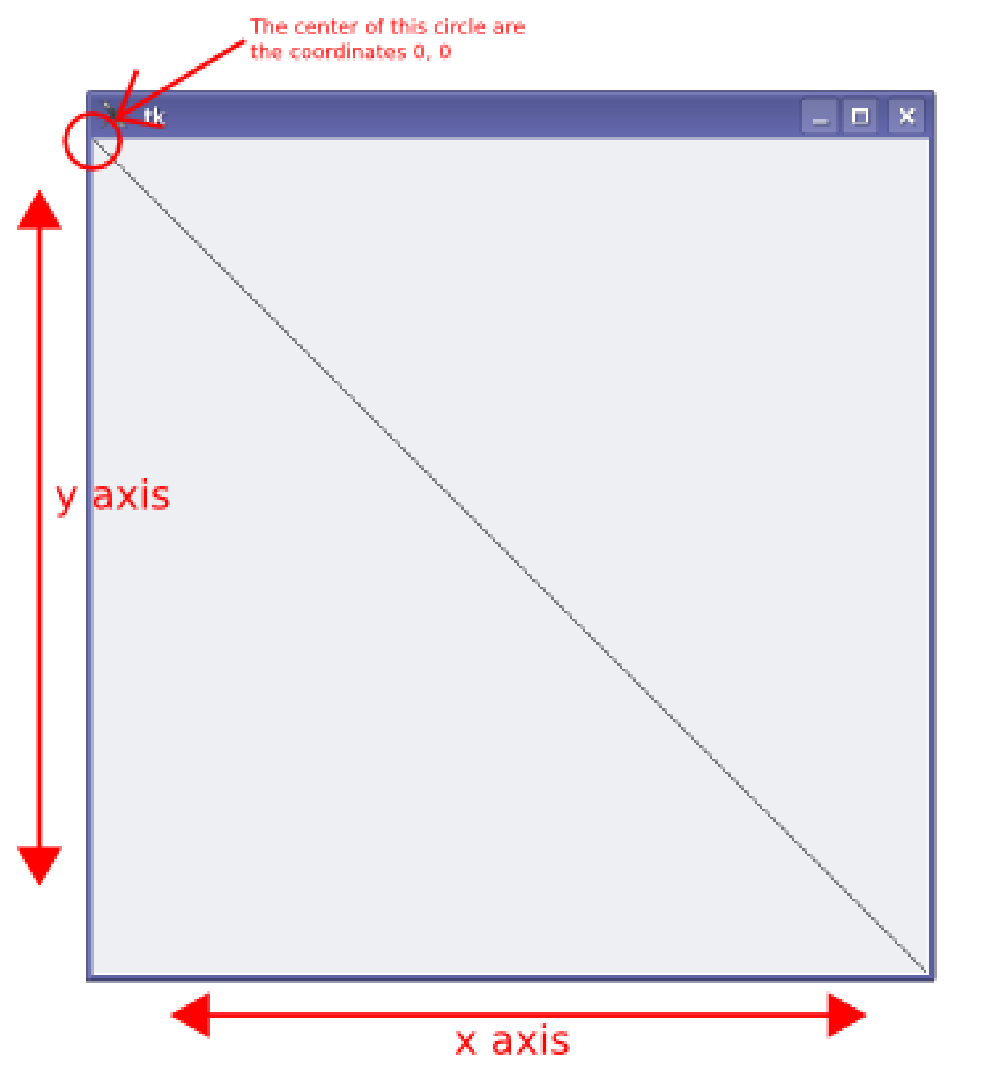
\includegraphics[width=80mm]{../en/figure32.eps}
\end{center}
\caption{Воображаемые оси координат на холсте}\label{fig32}
\end{figure}

Мы сделали холст размером 500 пикселей шириной и 500 высотой, так что координаты его правого нижнего угла — 500 и 500. Линию, которая есть на рисунке \ref{fig32}, можно нарисовать, указав координаты начальной точки: 0, 0 — и конечной точки: 500, 500\index{модули!tkinter!create\_line}:

\begin{listing}
\begin{verbatim}
>>> from tkinter import *
>>> tk = Tk()
>>> canvas = Canvas(tk, width=500, height=500)
>>> canvas.pack()
>>> canvas.create_line(0, 0, 500, 500)
\end{verbatim}
\end{listing}

У каждой точки всегда первая координата — по горизонтали ($x$), а вторая — по вертикали ($y$).

Если бы мы хотели добиться того же самого от черепашки, пришлось бы говорить ей гораздо больше всего:

\begin{listing}
\begin{verbatim}
>>> import turtle
>>> turtle.setup(width=500, height=500)
>>> t = turtle.Pen()
>>> t.up()
>>> t.goto(-250,250)
>>> t.down()
>>> t.goto(500,-500)
\end{verbatim}
\end{listing}

Рисовать линию при помощи \code{tkinter} уже проще, чем прибегая к услугам черепашки. А помимо рисования линий \code{tkinter} может исполнять для нас много разных других функций, про некоторые из которых мы сейчас поговорим.

\section{Нарисуем прямоугольники}

Когда мы объясняли черепашке, что нам нужен на экране прямоугольник, мы говорили ей продвинуться вперёд, повернуться, ещё продвинуться, ещё повернуться — и так далее. В результате всего этого получался квадрат или прямоугольник — смотря на сколько мы говорили черепашке двигаться вперёд. \code{tkinter}'у нам нужно просто сказать, что мы хотим видеть прямоугольник, и задать координаты его углов:

\begin{listing}
\begin{verbatim}
>>> from tkinter import *
>>> tk = Tk()
>>> canvas = Canvas(tk, width=400,height=400)
>>> canvas.pack()
>>> canvas.create_rectangle(10, 10, 50, 50)
1
\end{verbatim}
\end{listing}

Здесь мы создали квадратный холст размером 400×400 пикселей и нарисовали на нём квадрат. Левый верхний угол этого квадрата имеет координаты (10, 10), то есть от него 10 пикселей до левой и до верхней границ холста. Правый нижний — координаты (50, 50).

Функция \code{create\_rectangle}\index{модули!tkinter!create\_rectange} напечатала нам на экран число 1: это номер фигуры на холсте, которую мы только что нарисовали. Потом нам пригодятся такие номера.

Функции \code{create\_rectangle} мы передали четыре параметра. Первая пара параметров — координаты левого верхнего угла прямоугольника, а вторая пара — координаты правого нижнего. Прямоугольники все получаются с горизонтальными и вертикальными сторонами, их нельзя повернуть, используя только эту функцию. Координаты левой верхней точки обычно обозначают как «x1» (горизонтальная координата) и «y1» (вертикальная координата). Координаты правой нижней точки обычно обозначают как «x2» и «y2».

Если мы увеличим координату x2, то получится прямоугольник:

\begin{listing}
\begin{verbatim}
>>> canvas.create_rectangle(100, 100, 300, 50)
\end{verbatim}
\end{listing}

Можно вытянуть квадрат в другую сторону, получится другой прямоугольник:

\begin{listing}
\begin{verbatim}
>>> canvas.create_rectangle(100, 200, 150, 350)
\end{verbatim}
\end{listing}

Последняя из команд дословно значит вот что: отступи на 100 точек вправо от границы холста (левой верхней), и 200 точек вниз. Потом нарисуй прямоугольник шириной 150 точек направо и высотой 350 точек вниз. В результате выполнения этой команды холст должен выглядеть, как на рисунке \ref{fig33}.

\begin{figure}
\begin{center}
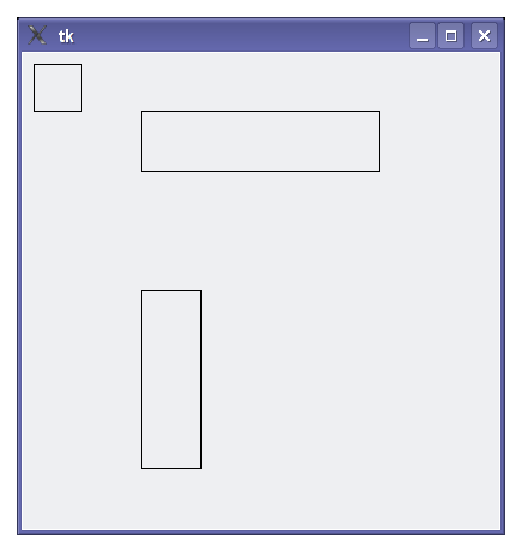
\includegraphics[width=80mm]{../en/figure33.eps}
\end{center}
\caption{Прямоугольнички от tkinter.}\label{fig33}
\end{figure}

Если теперь тебе в какой-то момент захочется очистить рисунок (то есть удалить всё с него), используй такую команду:
\begin{listing}
\begin{verbatim}
>>> canvas.delete('all')
\end{verbatim}
\end{listing}

Можем теперь попробовать нарисовать геометрическую абстрактную картинку, заполнив холст кучей разных прямоугольников. Для этого нам пригодится модуль \code{random}\index{модули!random}. Вначале его надо импортировать:

\begin{listing}
\begin{verbatim}
>>> import random
\end{verbatim}
\end{listing}

Кроме того, для удобства создадим функцию, которая будет нам рисовать прямоугольник случайного размера в случайном месте. Для этого потребуется вызвать функцию \code{randrange}\index{модули!random!randrange}:

\begin{listing}
\begin{verbatim}
>>> def random_rectangle(width, height):
...     x1 = random.randrange(width)
...     y1 = random.randrange(height)
...     x2 = random.randrange(x1 + random.randrange(width))
...     y2 = random.randrange(y1 + random.randrange(height))
...     canvas.create_rectangle(x1, y1, x2, y2)
\end{verbatim}
\end{listing}

В первых двух строчках функции мы создаём переменные, определяющие левый верхний угол будущего прямоугольника. Функция \code{randrange} возвращает нам число от 0 до числа, которое мы ей передали как параметр (не включая это число). Она умеет ещё несколько других параметров принимать, подробнее об этом написано в приложении \ref{app:afewpythonmodules}. Если мы вызовем \code{randrange(10)}, то получим какое-то число от 0 до 9. Если вызовем \code{randrange(100)} — какое-то число от 0 до 99.

В следующих двух строках мы таким же образом определяем координаты правого нижнего угла нашего прямоугольника (может, это даже будет квадрат, кто знает): добавляем случайные числа к каждой из координат левого верхнего угла. После всего этого мы наконец создаём прямоугольник при помощи функции \code{create\_rectangle}.

Можешь попробовать, как эта функция работает:

\begin{listing}
\begin{verbatim}
>>> random_rectangle(400, 400)
\end{verbatim}
\end{listing}

Можно ещё сделать сотню разных прямоугольничков:

\begin{listing}
\begin{verbatim}
>>> for x in range(0, 100):
...     random_rectangle(400, 400)
\end{verbatim}
\end{listing}

Получается куча линий, что-то вроде того, что на рисунке \ref{fig34}.

\begin{figure}
\begin{center}
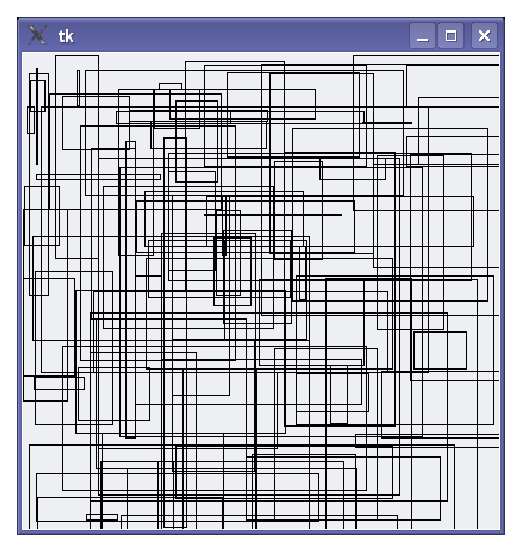
\includegraphics[width=80mm]{../en/figure34.eps}
\end{center}
\caption{Прямоугольный беспорядок.}\label{fig34}
\end{figure}

Ты можешь помнить, что в последней главе мы говорили черепашке, каким цветом рисовать, задавая долю каждого из трёх цветов: красного, синего и зелёного. Используя \code{tkinter}, можно задать цвет примерно так же, но записав это по-другому. Прежде всего, давай научим нашу функцию рисовать разноцветно:


\begin{listing}
\begin{verbatim}
>>> def random_rectangle(width, height, fill_colour):
...     x1 = random.randrange(width)
...     y1 = random.randrange(height)
...     x2 = random.randrange(x1 + random.randrange(width))
...     y2 = random.randrange(y1 + random.randrange(height))
...     canvas.create_rectangle(x1, y1, x2, y2, fill=fill_colour)
\end{verbatim}
\end{listing}

Функции \code{create\_rectangle} можно передать параметр \code{fill}, значение которого — цвет, которым заполнять прямоугольник. Теперь можно сделать разноцветный беспорядок:

\begin{listing}
\begin{verbatim}
>>> random_rectangle(400, 400, 'green')
>>> random_rectangle(400, 400, 'red')
>>> random_rectangle(400, 400, 'blue')
>>> random_rectangle(400, 400, 'orange')
>>> random_rectangle(400, 400, 'yellow')
>>> random_rectangle(400, 400, 'pink')
>>> random_rectangle(400, 400, 'purple')
>>> random_rectangle(400, 400, 'violet')
>>> random_rectangle(400, 400, 'magenta')
>>> random_rectangle(400, 400, 'cyan')
\end{verbatim}
\end{listing}

Не пугайся, если некоторые функции не выполнились, а только напечатали сообщение об ошибке. Какие именно цвета \code{tkinter} узнаёт по названию, зависит от операционной системы (Windows, Mac OS, Linux) и от версии этого пакета. Тут-то и встаёт вопрос: как нарисовать  цвет, названия которого \code{tkinter} не знает? Примерно так же, как мы просили этого от черепашки: сказать, сколько в этом цвете красного, зелёного и синего. Только \code{tkinter} ждёт этого записанного в другом виде. Например, золотой цвет (100\% красного, 85\% зелёного и 0\% синего) задаётся вот так:

\begin{listing}
\begin{verbatim}
>>> random_rectangle(400, 400, '#ffd800')
\end{verbatim}
\end{listing}

Эти цифры и буквы после решёточки — шестнадцатеричные\footnote{Шестнадцатеричных цифр 16, по порядку от 0 до 9 и потом a, b, c, d, e, f.}. Первые две цифры — ff — соответствуют красному (максимальное значение для него), вторые две — d8 — зелёному, а последние две — 00 — синему (его нет). Разбираться в этом всём нет большой необходимости, потому что можно просто написать функцию, которая будет нам выдавать строки, понятные \code{tkinter}'у из того, что понятно нам. Функция эта будет выглядеть вот так:

\begin{listing}
\begin{verbatim}
>>> def hexcolor(red, green, blue):
...     red = 255*(red/100.0)
...     green = 255*(green/100.0)
...     blue = 255*(blue/100.0)
...     return '#%02x%02x%02x' % (red, green, blue)
\end{verbatim}
\end{listing}

Если попросить её закодировать золотистый цвет, то получится…

\begin{listing}
\begin{verbatim}
>>> print(hexcolor(100, 85, 0))
#ffd800
\end{verbatim}
\end{listing}

… как раз то, что надо.

Или можно попросить её закодировать сиреневый цвет (98\% красного, 1\% зелёного, 77\% синего):

\begin{listing}
\begin{verbatim}
>>> print(hexcolor(98, 1, 77))
#f902c4
\end{verbatim}
\end{listing}

Теперь этот цвет можно передавать в нашу функцию \code{random\_rectangle}:

\begin{listing}
\begin{verbatim}
>>> random_rectangle(400, 400, hexcolor(98, 1, 77))
\end{verbatim}
\end{listing}

\begin{figure}
\begin{center}
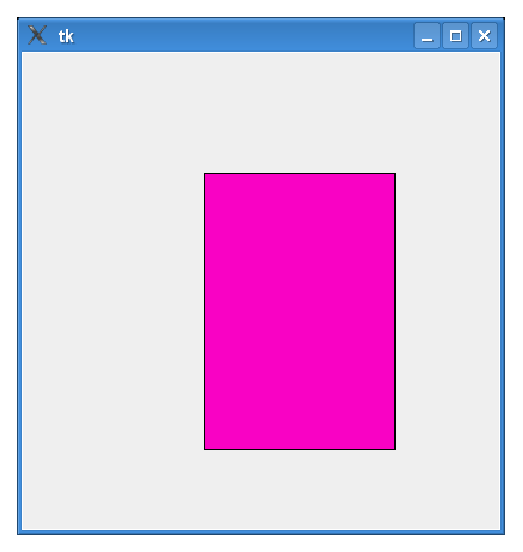
\includegraphics[width=60mm]{../en/figure35.eps}
\end{center}
\caption{Сиреневый прямоугольник.}\label{fig35}
\end{figure}

\section{Нарисуем дугу}

Дуга — это часть эллипса (ну или круга — круг тоже является эллипсом), но чтобы нарисовать её при помощи \code{tkinter}, надо задать координаты прямоугольника — левого верхнего и правого нижнего угла, как и раньше. Это может показаться странным, но смысл тут вот в чём: мы задаём прямоугольник, в который вписан эллипс, чью дугу нам надо нарисовать, как это нарисовано на картинке \ref{fig36}. Помимо прямоугольника мы говорим ещё, какую часть дуги рисовать: 359 — значит весь эллипс, 180 — значит половину эллипса, а 0 — совсем ничего.

Чтобы нарисовать картинку \ref{fig36}, подойдёт вот такой код\index{модули!tkinter!create\_arc}:

\begin{listing}
\begin{verbatim}
canvas.create_arc      (10, 10, 200, 100, extent=200, style=ARC)
canvas.create_rectangle(10, 10, 200, 100)
\end{verbatim}
\end{listing}

\begin{figure}
\begin{center}
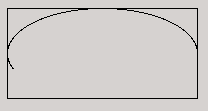
\includegraphics[width=80mm]{figure36.png}
\end{center}
\caption{Дуга в прямоугольнике.}\label{fig36}
\end{figure}

Параметры функции \code{create\_arc} такие: сначала мы задаём четыре координаты прямоугольника (так же, как обычно); потом мы говорим, сколько градусов дуги нам надо рисовать (от 0 до 359); потом мы говорим, что мы хотим видеть только саму дугу\footnote{Другие варианты — \code{style=PIESLICE} и \code{style=CHORD}.}. Ниже для примера нарисованы дуги с разным количеством градусов, результат — на рисунке \ref{fig37}:

\begin{listing}
\begin{verbatim}
>>> canvas.create_arc(10, 10, 200, 80, extent=45, style=ARC)
>>> canvas.create_arc(10, 80, 200, 160, extent=90, style=ARC)
>>> canvas.create_arc(10, 160, 200, 240, extent=135, style=ARC)
>>> canvas.create_arc(10, 240, 200, 320, extent=180, style=ARC)
>>> canvas.create_arc(10, 320, 200, 400, extent=359, style=ARC)
\end{verbatim}
\end{listing}

\begin{figure}
\begin{center}
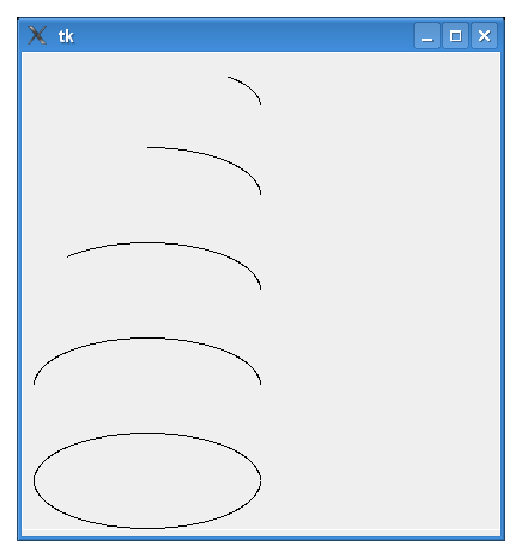
\includegraphics[width=80mm]{../en/figure37.eps}
\end{center}
\caption{Дуги разной длины.}\label{fig37}
\end{figure}

\section{Нарисуем эллипс}

Последняя из команд в предыдущем примере рисует аккурат целый эллипс. Чтобы рисовать эллипсы, есть и специальная команда, покороче: \code{create\_oval}\footnote{Эллипс — частный случай овала; так же, как окружность — частный случай эллипса.}. Как и для рисования дуги, для рисования эллипса надо задать ограничивающий прямоугольник. Например, вот такой:

\begin{listing}
\begin{verbatim}
>>> tk = Tk()
>>> canvas = Canvas(tk, width=400,height=400)
>>> canvas.pack()
>>> canvas.create_oval(1, 1, 300, 200)
\end{verbatim}
\end{listing}

Этот пример рисует эллипс в воображаемом прямоугольнике который занимает пространство от точки (1, 1) до точки (300, 200). Если мы теперь нарисуем прямоугольник с теми же координатами, то увидим, что эллипс как раз аккуратно в него вписан (и получится у нас рисунок \ref{fig38}):

\begin{listing}
\begin{verbatim}
>>> canvas.create_rectangle(1, 1, 300, 200, outline="#ff0000")
\end{verbatim}
\end{listing}

\begin{figure}
\begin{center}
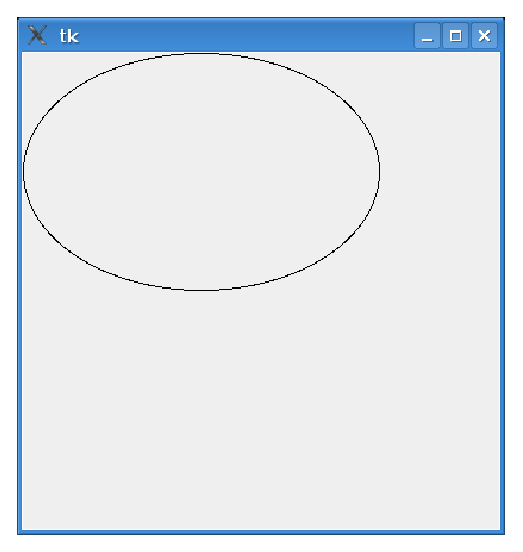
\includegraphics[width=80mm]{../en/figure38.eps}
\end{center}
\caption{Эллипс}\label{fig38}
\end{figure}

\begin{figure}
\begin{center}
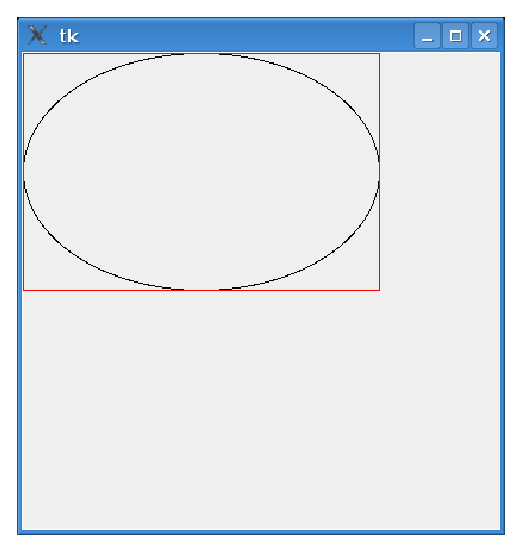
\includegraphics[width=80mm]{../en/figure39.eps}
\end{center}
\caption{Эллипс в рамочке.}\label{fig39}
\end{figure}

Чтобы нарисовать окружность, нам нужно в качестве ограничивающего прямоугольника задать квадрат (как на картинке \ref{fig40}):

\begin{listing}
\begin{verbatim}
>>> tk = Tk()
>>> canvas = Canvas(tk, width=400,height=400)
>>> canvas.pack()
>>> canvas.create_oval(1, 1, 300, 300)
\end{verbatim}
\end{listing}

\begin{figure}
\begin{center}
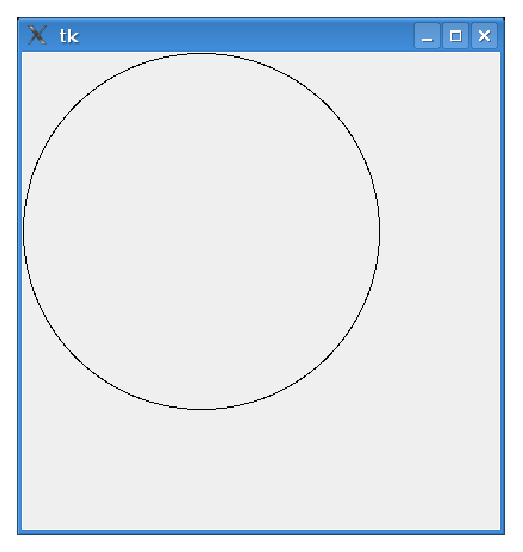
\includegraphics[width=80mm]{../en/figure40.eps}
\end{center}
\caption{Окружность}\label{fig40}
\end{figure}

\section{Нарисуем многоугольник}\index{modules!tkinter!create\_polygon}

Многоугольник — это какая-то геометрическая фигура с углами, у которой больше двух сторон. Треугольники, прямоугольники, пятиугольники — это всё примеры многоугольников. Помимо этих правильных форм, можно создавать и более неуклюжие фигуры. Для этого есть функция \code{create\_polygon}. Ей нужно передать столько пар координат, сколько вершин у нашего многоугольника, а она соединит все эти вершины и, если попросить, закрасит получившуюся фигуру.

Начнём с треугольника. У него три вершины, у каждой по две координаты; закрашивать его мы не хотим; а линии пусть рисуются чёрными. Всё это на питоньем языке выглядит так (а в результате получается рисунок \ref{fig41}):

\begin{listing}
\begin{verbatim}
>>> from tkinter import *
>>> tk = Tk()
>>> canvas = Canvas(tk, width=400,height=400)
>>> canvas.pack()
>>> canvas.create_polygon(10, 10, 100, 10, 100, 50, fill="", outline="black")
\end{verbatim}
\end{listing}

\begin{figure}
\begin{center}
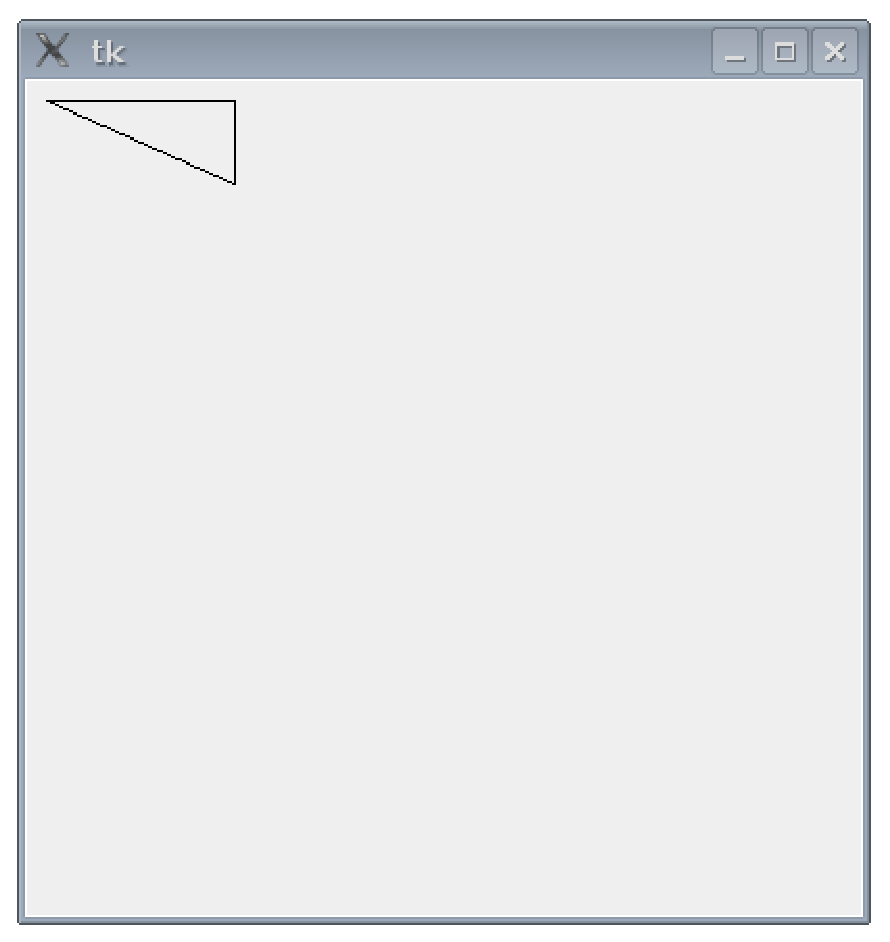
\includegraphics[width=80mm]{../en/figure41.eps}
\end{center}
\caption{Треуголник.}\label{fig41}
\end{figure}

Чтобы нарисовать какой-то четырёхугольник, надо передать уже восемь координат (четыре пары):

\begin{listing}
\begin{verbatim}
>>> canvas.create_polygon(200, 10, 240, 30, 120, 100, 140, 120, fill="", outline="black")
\end{verbatim}
\end{listing}

На рисунке \ref{fig42} есть треугольник и ещё четырёхугольник (который выглядит как пара треугольников вместе).

\begin{figure}
\begin{center}
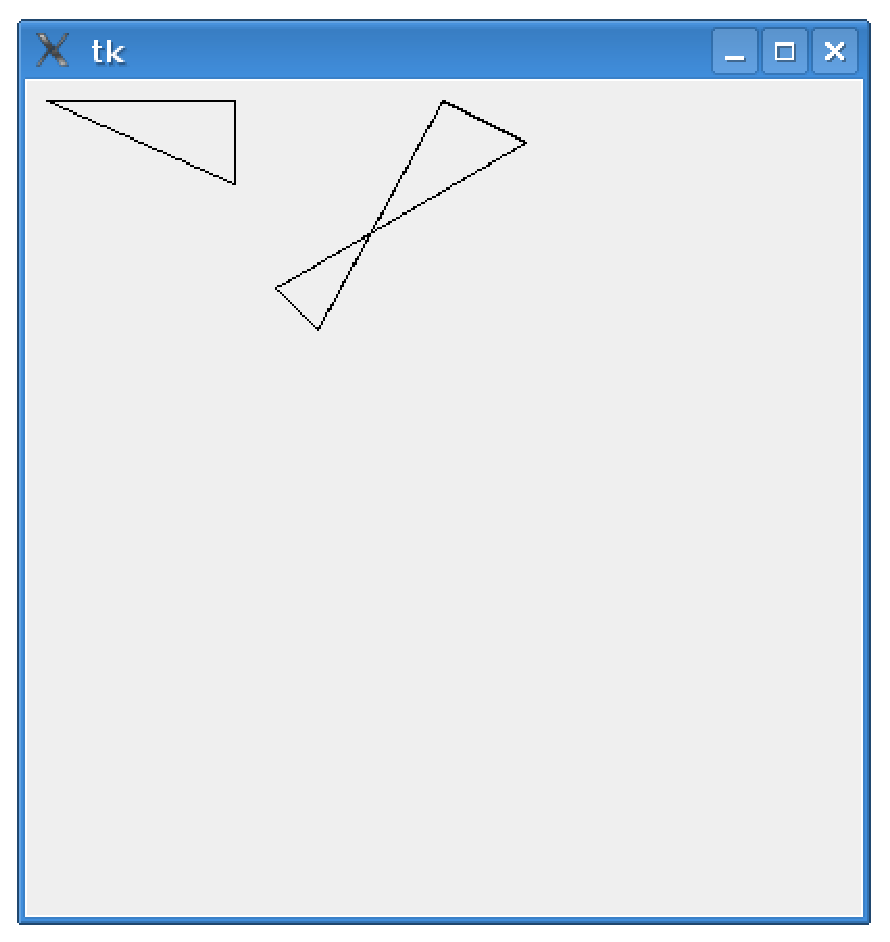
\includegraphics[width=80mm]{../en/figure42.eps}
\end{center}
\caption{Треугольник. И четырёхугольник.}\label{fig42}
\end{figure}

\section{Нарисуем картину}

Питону можно сказать вывести на экран целую картинку сразу (например, фотографию). Для этого ему нужно сказать загрузить в память картинку и вывести её на холст при помощи функции \code{create\_image}\index{модули!tkinter!create\_image}:

\begin{listing}
\begin{verbatim}
1. >>> from tkinter import *
2. >>> tk = Tk()
3. >>> canvas = Canvas(tk, width=400, height=400)
4. >>> canvas.pack()
5. >>> myimage = PhotoImage(file='test.gif')
6. >>> canvas.create_image(0, 0, image=myimage, anchor=NW)
\end{verbatim}
\end{listing}

В первых четырёх строчках мы, как всегда, создаём холст. В пятой строке загружаем картинку из файла «test.gif» в переменную myimage. В последней строке говорим  нарисовать эту картинку в левом верхнем углу холста.

Чтобы всё получилось, картинка должна лежать там, где Питон её ищет. Спросить у него, где он ищет, можно, вызвав функцию \code{getcwd()} из модуля \code{os}\index{модули!os}:

\begin{listing}
\begin{verbatim}
>>> import os
>>> print(os.getcwd())
\end{verbatim}
\end{listing}

\begin{WINDOWS}
Наверное, Питон напечатает тебе что-то вроде «c:\\Python30».
\end{WINDOWS}

\begin{MAC}
Скорее всего, Питон напечатает тебе что-то вроде «/Users/yourname», заменив yourname на имя пользователя. Например, если твоего пользователя зовут john, то на экране появится «/Users/john».
\end{MAC}

\begin{LINUX}
Скорее всего, Питон напечатает тебе что-то вроде «/home/yourname», заменив yourname на имя пользователя. Например, если твоего пользователя зовут john, то на экране появится «/home/john».
\end{LINUX}

Положи нужную тебе картинку в эту папку и запусти код из примера выше. Если всё сделать правильно, то получится-то что-нибудь наподобие рисунка \ref{fig43}.

\begin{figure}
\begin{center}
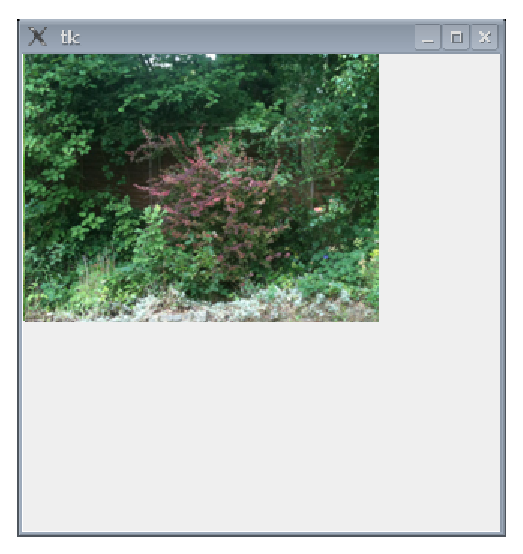
\includegraphics[width=80mm]{../en/figure43.eps}
\end{center}
\caption{Фотография.}\label{fig43}
\end{figure}

Функция \code{PhotoImage} может загружать файлы форматов gif, ppm и pgm. Если тебе захочется загрузить другой файл — скажем, jpg или png, — то тебе пригодится модуль, который это умеет. Скажем, Python Imaging Library (PIL)\footnote{Его можно загрузить здесь: \url{http://www.pythonware.com/products/pil/index.htm}} — этот модуль  умеет загружать всевозможные картинки, а также обрезать их, менять цвета, поворачивать и всё в таком духе. Я не буду объяснять, как установить этот модуль, для этого бы потребовалось написать много того, что не относится к познаванию Питона.

\section{Простая анимация}\index{модули!tkinter!простая анимация}

До сих пор мы рисовали неподвижные картинки. Этим возможности Питона не ограничиваются: \code{Tk} может нарисовать нам и движущиеся фигуры, хотя это не его сильная сторона. Например, мы вполне можем от него добиться закрашенного треугольничка, бегающего по экрану. Вот код для этого:

\begin{listing}
\begin{verbatim}
1.  >>> import time
2.  >>> from tkinter import *
3.  >>> tk = Tk()
4.  >>> canvas = Canvas(tk, width=400, height=400)
5.  >>> canvas.pack()
6.  >>> canvas.create_polygon(10, 10, 10, 60, 50, 35)
7.  1
8.  >>> for x in range(0, 60):
9.  ...     canvas.move(1, 5, 0)
10. ...     tk.update()
11. ...     time.sleep(0.05)
\end{verbatim}
\end{listing}

В тот момент, когда ты нажмёшь Enter после последней строки, треугольничек задвигается. Он на полпути изображён на рисунке \ref{fig44}.

\begin{figure}
\begin{center}
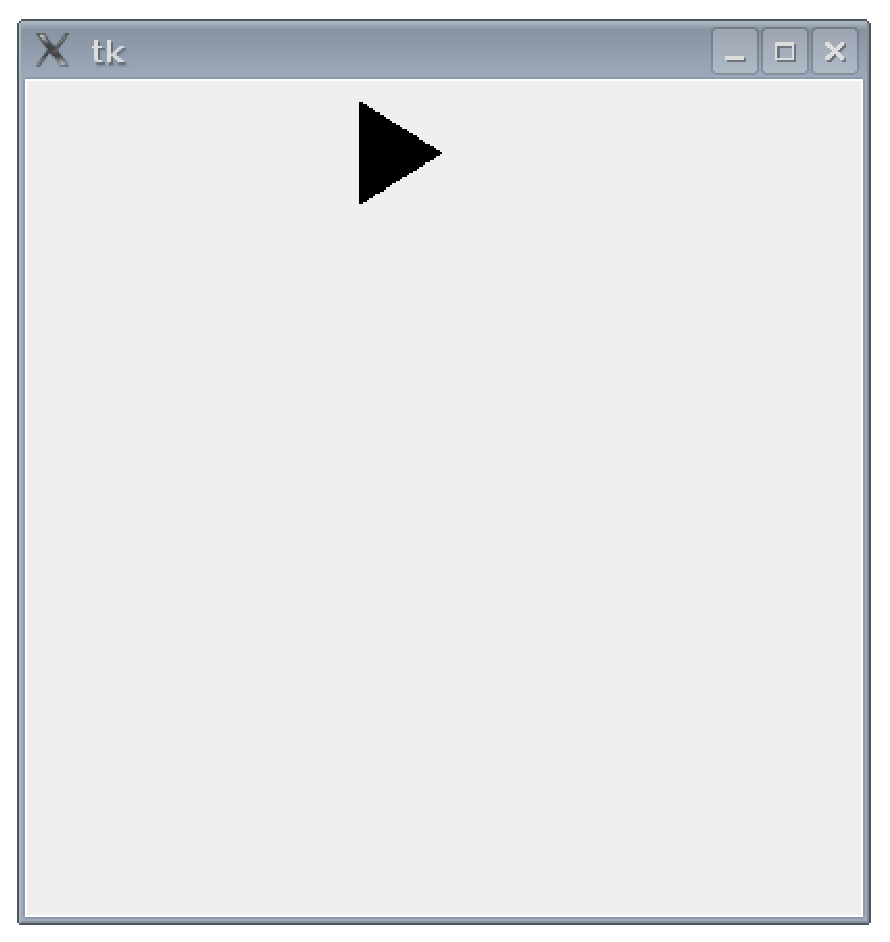
\includegraphics[width=80mm]{../en/figure44.eps}
\end{center}
\caption{Треугольничек во время движения по экрану.}\label{fig44}
\end{figure}

\par
\emph{Как это работает?}
\par

Строки с 1 по 5 мы уже видели раньше — это просто настройка холста, — а в строке 6 мы создаём треугольник. В строке 7 Питон напечатал номер треугольника — это первая фигура на холсте. В строке 8 мы создаём цикл из 60 шагов.

Строки с 9 по 11 объясняют Питону, что треугольник должен двигаться. Функция \code{move} объекта \code{canvas} передвигает зажанный объект, прибавляя значения к его координатам x и у. В строке 9 мы просим её двигать объект №1 на 5 пикселей вправо и на 0 пикселей вбок. Если бы мы хотели, чтобы треугольник полз влево, нам бы стоило написать вот как: \code{canvas.move(1, -5, 0)}\index{модули!tkinter!move}.

Функция \code{update} в следующей строке говорит Питону перерисовать изображение. Без неё он бы сперва дождался конца цикла и потом нарисовал треугольник в его новом месте, а движения треугольника к новому месту мы бы не увидели. Наконец, в строке 11 мы говорим Питону притормозить на 1/20 секунды перед следующим шагом. Если мы скажем тормозить большее время, то треугольник будет двигаться рывками.

Можно изменить этот код так, чтобы треугольник двигался наискосок через холст. Например так: закрой графическое окно с треугольником и введи в консоль Питона следующий код:

\begin{listing}
\begin{verbatim}
>>> import time
>>> tk = Tk()
>>> canvas = Canvas(tk, width=400, height=400)
>>> canvas.pack()
>>> canvas.create_polygon(10, 10, 10, 60, 50, 35)
1
>>> for x in range(0, 60):
...     canvas.move(1, 5, 5)
...     tk.update()
...     time.sleep(0.05)
...
\end{verbatim}
\end{listing}

Рисунок \ref{fig45} показывает треугольник на полпути к финишу. Можно вернуть треугольник к началу таким кодом:

\begin{listing}
\begin{verbatim}
>>> import time
>>> for x in range(0, 60):
...     canvas.move(1, -5, -5)
...     tk.update()
...     time.sleep(0.05)
\end{verbatim}
\end{listing}

\begin{figure}
\begin{center}
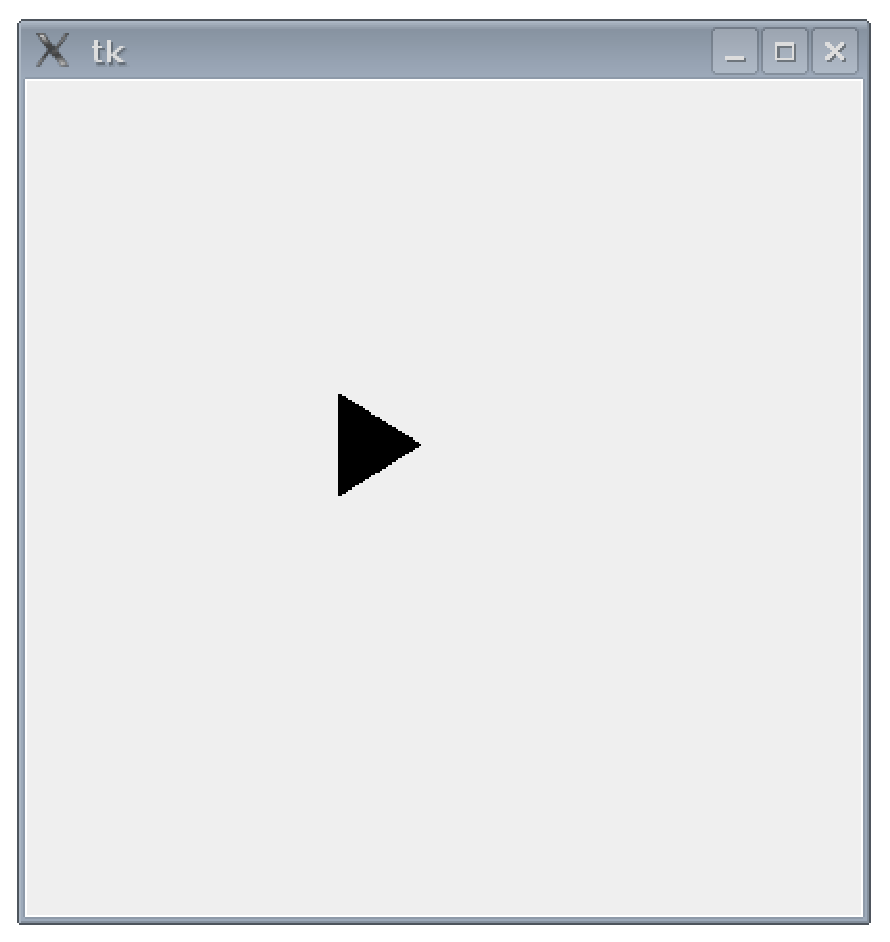
\includegraphics[width=80mm]{../en/figure45.eps}
\end{center}
\caption{Треугольник на полпути к низу экрана.}\label{fig45}
\end{figure}

\section{Реагируем на события…}\index{модули!tkinter!события}

Мы можем сделать так, чтобы треугольник бегал по экрану не просто как его нравится, а в ответ на наши нажатия клавиш. Нажатия клавиш для Питона — один из видов событий, и на них можно реагировать. Ещё события — это движение мыши, перемещение или закрытие окна. Можно указать \code{Tk}, что делать, когда каждое из событий возникает. Первым делом для этого надо создать функцию, которая и будет вызываться в случае чего. Допустим, мы хотим подвинуть треугольник. Вот функция для этого:

\begin{listing}
\begin{verbatim}
>>> def movetriangle(event):
...     canvas.move(1, 5, 0)
\end{verbatim}
\end{listing}

У функции должен быть один параметр, а именно — событие. Так \code{Tk} сообщает нам, что именно произошло — это пригодится, если одна и та же функция реагирует на много разных событий, но немножко по-разному. Теперь эту функцию можно привязать к событию нажатия клавиши Enter, используя функцию \code{bind\_all}\index{modules!tkinter!bind\_all}. Вот так:

\begin{listing}
\begin{verbatim}
>>> from tkinter import *
>>> tk = Tk()
>>> canvas = Canvas(tk, width=400, height=400)
>>> canvas.pack()
>>> canvas.create_polygon(10, 10, 10, 60, 50, 35)
>>> def movetriangle(event):
...     canvas.move(1, 5, 0)
...
>>> canvas.bind_all('<KeyPress-Return>', movetriangle)
\end{verbatim}
\end{listing}

Первым параметром функции \code{bind\_all} передаётся название события. \\«\code{<KeyPress-Return>}» значит «нажата клавиша Enter (её по-английски иногда называют Return). Вторым параметром мы сообщаем функции, что вызывать, если это событие случилось. Если этот код запустить и щёлкнуть мышкой по холсту с треугольником (чтобы система поняла, что все следующие нажатия клавиш надо отправлять именно ему), то пока нажата клавиша Enter, треугольник будет двигаться.

Теперь мы можем заставить треугольник двигаться туда, куда мы хотим. А говорить ему, куда мы хотим, мы будем, нажимая стрелки на клавиатуре. Функция ниже как раз так и работает: например, если нажать стрелку вниз, то треугольник уползёт на три пикселя вниз:

\begin{listing}
\begin{verbatim}
>>> def movetriangle(event):
...     if event.keysym == 'Up':
...         canvas.move(1, 0, -3)
...     elif event.keysym == 'Down':
...         canvas.move(1, 0, 3)
...     elif event.keysym == 'Left':
...         canvas.move(1, -3, 0)
...     else:
...         canvas.move(1, 3, 0)
\end{verbatim}
\end{listing}

У параметра \code{event}, который передаётся в функцию, есть несколько \emph{полей}, то есть значений внутри. Одно из них мы как раз используем: это \code{keysym}. В реальной жизни у разных вещей тоже есть всякие свойства: например, у неба есть цвет, и значение этого свойства — «голубой». А у воды есть свойство «температура», значением которой может быть число — чему она равна в градусах.

Так вот, у нашего события есть свойство: какая клавиша была нажата. Ориентируясь на значение этого свойства (или поля, это разные названия одного и того же), мы выбираем, куда двигать треугольник. Допустим, если нажата была клавиша вверх (по-английски — «Up»), то нам нужно подвинуть фигуру №1 (наш треугольник) на 0 пикселей вправо и на 3 пикселя вверх. Ну и в остальные стороны похожим образом.

Осталось нам назначить эту функцию обработчиком событий от нажатий четырёх стрелок, вот так:

\begin{listing}
\begin{verbatim}
>>> from tkinter import *
>>> tk = Tk()
>>> canvas = Canvas(tk, width=400, height=400)
>>> canvas.pack()
>>> canvas.create_polygon(10, 10, 10, 60, 50, 35)
1 
>>> def movetriangle(event):
...     if event.keysym == 'Up':
...         canvas.move(1, 0, -3)
...     elif event.keysym == 'Down':
...         canvas.move(1, 0, 3)
...     elif event.keysym == 'Left':
...         canvas.move(1, -3, 0)
...     else:
...         canvas.move(1, 3, 0)
... 
>>> canvas.bind_all('<KeyPress-Up>', movetriangle)
>>> canvas.bind_all('<KeyPress-Down>', movetriangle)
>>> canvas.bind_all('<KeyPress-Left>', movetriangle)
>>> canvas.bind_all('<KeyPress-Right>', movetriangle)
\end{verbatim}
\end{listing}

Если запустить этот код, то треугольник будет двигаться в ту сторону, куда мы попросим.

\newpage